%%%%%%%%%%%%%%%%%%%%%%%%%%%%%%%
% Tradeoff from problem chapter
%%%%%%%%%%%%%%%%%%%%%%%%%%%%%%%
\section{Tradeoff}
Note: tradeoff between accuracy and computational cost $\rightarrow$ mobile phone dilemma

When determining whether automation is an improvement four aspects have to be examined.
These are time, costs, quality and flexibility.
The aspects build a quadrangle that is based on the optimizing trade-off between the
factors~\cite{dumas_fundamentals_2013}.

Without software supporting the task of reading the name of the picture and typing it into
the system, can take long seconds, whereas a trained \ac{DL} model could complete the task
in a mere instant.
Therefor automisation via \ac{DL} should improve the efficiency of the process when compared to
manually reading and typing the information off the image.

Training costs for a \ac{DL} model are very high due to the computing intensive
backpropagation algorithm that tunes the network to the data.
But the usage cost is low.
For manual labor the opposite is the case as training a person to type in a label is done quickly
and labor costs are high in comparison to the expenses for running the model.

Both \ac{DL} models and human labor are not 100\% accurate.
The question is whether the model can be as accurate or even better than its human counterpart.
This is especially interesting when it is applied in the real world where it might have to do good
in subpar situations.
An example is bad image quality.

Flexibility is concerned with how well a process can adjust to changing requirements.
A set of new equipment names that have to be included can pose a problem to a \ac{DL} model
because it is not trained for the new data.
A human on the other hand should not have any problems in this regard.

The main concern for the solution's efficacy is whether it is accurate enough.
Therefor this work focuses on this aspect in particular.


%%%%%%%%%%%%%%%%%%%%%%%%%%%%%%%%%%
% Problem chapter: with FR and NFR
%%%%%%%%%%%%%%%%%%%%%%%%%%%%%%%%%%

% Def Requirements / what to expect
For traditional software projects requirements engineering classifies requirements into
two categories~\cite{zowghi_requirements_2014}.
\Acp{FR} specify functionality that users can experience~\cite{noauthor_ieee_1998}.
Other requirements that are relevant to the project in a way that shapes the target system,
defines the development process and manages the development project are refered to as
\acp{NFR}~\cite{kotonya_requirements_1998,chung_non-functional_2009}.
For \ac{ML} and thus \ac{DL} projects, data directly influences the performance of the solution.
This results in the need to specify \acp{DR} for data that is used
in conjunction with the \ac{DL} system~\cite{vogelsang_requirements_2019}.

% keep requirements such as maintenance (encapsulation, modularity), development, ...??

% functional requirements
The basic functionality can be described as extraction of textual data from images.
The relevant text information is framed by a label.
The label contains printed text which can be structured and spaced differently from label to
label (see figure~\ref{fig:examples}).
The text, spacing and structure carries semantic information which can be important for later
processing in the scope of a business process.
The goal is to extract the text and preserve semantics from structure and space.
This means text and the respective coordinates, height, width and a possible rotation angle must
be output as the result~\cite{yang_learning_2021}.
Those values can then be transformed into other formats such as JSON or HTML as needed.
The images can contain arbitrary alpha-numeric strings (see figure~\ref{fig:examples}).
This results in the requirement that the \ac{DL} model has to be able to recognize sequences that
are not part of a predefined lexicon~\cite{ghosh_visual_2017}.
% performance, change reliability to performance after checking source


% non-functional requirements
% find sources
The \acp{NFR} that derive from the intended use for the solution with mobile phones are led by
power aspects.
Not only are mobile phones limited by a finite battery but also by computational power.
In this regard \acp{NN} can be challenging because they often have an immense amount of parameters
which are computationally demanding and can therefore also be a burden for the phone's power supply.
Therefore, finding an approach which reduces computational complexity is important.
The solution will be used on mobile phones that have no access to the internet.
This is why the extraction must work offline.
Varying aspect ratios in images and such diversities can increase the requirements for preprocessing.
Depending on the approach the complexity can change i.e.\ decrease thus making it more viable.

% data requirements
% focus more on annotation, costs or difference for different algorithms
\acp{DR} encompass the data that is required in order to train, tune and test a \ac{DL}
system~\cite{vogelsang_requirements_2019}.
Difficulties arise from the amount of data needed to train a \ac{DL} model and from the need to
annotate the data for supervised learning~\cite{nowruzi_how_2019}.
However, it is possible to pretrain a model on a dataset for a related task.
The pretrained model can then be fine tuned to fit the actual task thus decreasing the needed size
in the data set that is specific to the problem~\cite{ouyang_factors_2016}.
This procedure allows for achieving good performance.
Additionally there's many available pretraining datasets that are labeled~\cite{ouyang_factors_2016}.
In the context of requirements, quantity refers to diversity of data~\cite{vogelsang_requirements_2019}.
When it comes to the quality of data there's three factors: completeness, consistency,
correctness.
These factors are especially important since better quality as a big influence on
performance~\cite{vogelsang_requirements_2019}.
% set into relation with data quantity? after certain amount of data convergence to value
%       but if quality better higher convergence
For completeness, it is important that the dataset that is used for finetuning contains all edge
cases that are relevant for the task~\cite{arpteg_software_2018, vogelsang_requirements_2019}.
`Consistency refers to the format and representation of data that should be the same in the dataset. Correctness refers to the degree to which you can rely on the data actually being
true'\cite{vogelsang_requirements_2019}.
As implementation and training a \ac{DL} model is not the subject of this theses these \ac{DR} are
not discussed in detail in the following chapters.
% add following
Relevant, Complete, Balanced, Accurate~\cite{ashmore_assuring_2021}

%%%%%%%%%%%%%%%%%%%%%%%%
% Transformer theory
%%%%%%%%%%%%%%%%%%%%%%%%%
\section{Transformers}
% look into \cite{kloss_learning_2016}
% either improve or remove
Of the most popular basic strucures for \acp{NN}, the transformers are the newest innovation.
The paper from~\cite{vaswani_attention_2017} introduced the transfomer architecture which is
build for processing sequence data and~\cite{dosovitskiy_image_2021} then introduced the vision
transformer (ViT).
\begin{figure}[ht]
    \centering
    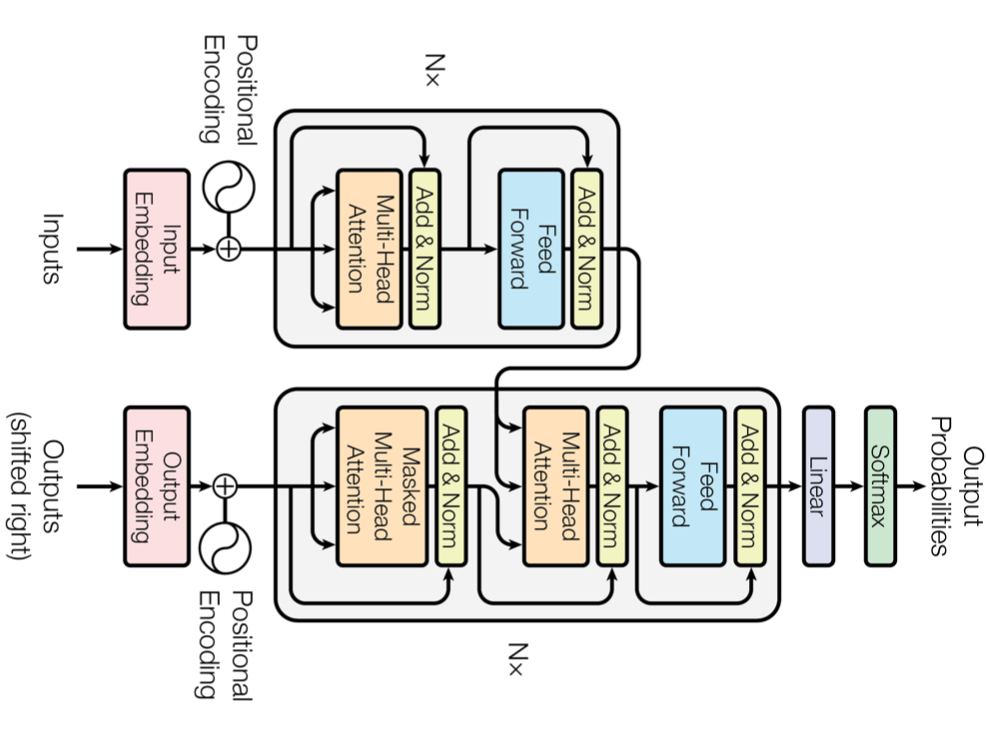
\includegraphics[width=0.8\textwidth]{img/Transformer-Vaswani-Attention-2017.png}
    \caption[Transformer architecture]{%
        Transformer model architecture~\citep{vaswani_attention_2017}\label{fig:transformer}
    }
\end{figure}
Explaining the inner workings of transformers in detail exceeds the scope of this thesis.
In the following the basic building blocks and their effects are described with the example of
translating a sentence.
Figure~\ref{fig:transformer} shows a transformer network at the abstraction level of components and
their alignment to build the network.
The network is made up of multiple multiple encoder and multiple decoder
blocks ($Nx$)~\citep{vaswani_attention_2017}.
The blocks are preceded by embedding and positional modules~\citep{vaswani_attention_2017}.
The embedding modules map a word to a vector, also interpreted as a point in space, where similar
words are close to each other~\citep{vaswani_attention_2017}.
An example for a embedding space is presented by~\cite{pennington_glove_2014}.
Because the placing of a word in a sentence can change the meaning, positional
encoding is added to the word embedding~\citep{vaswani_attention_2017}.
The encoder and decoder blocks contain multi-head attention modules and feedforward networks.
They also contain skip connections (introduced with residual block~\citep{he_deep_2015}) and layer
normalization~\citep{vaswani_attention_2017} which helps with training the network and to keep it
stable~\citep{liu_rethinking_2021}.
A multi-head attention block calculates which words (by now embedded) of the input are
important for each other word.
The attention is calculated by a scaled dot product (see
Figure~\ref{fig:transformer-dot-product})~\citep{vaswani_attention_2017}.
\begin{figure}[ht]
    \centering
    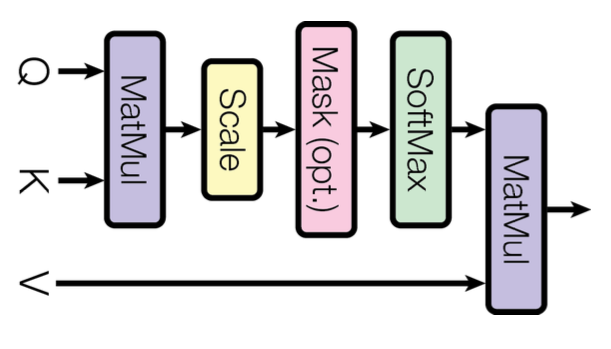
\includegraphics[width=0.5\textwidth]{img/Transformer-Scaled-Dot-Product-Vasani-Attention-2017.png}
    \caption[Computation of an attention mechanism]{%
        Scaled dot product used to compute attention
        vectors~\citep{vaswani_attention_2017}\label{fig:transformer-dot-product}
    }
\end{figure}
% use ihttps://github.com/janosh/tikz/tree/main/assets/self-attention nstead
This is calculated multiple times (hence the term multi-head) and the results are merged by
concatenation and a subseding linear layer~\citep{vaswani_attention_2017}.
This allows the model to use different representations of the
information~\citep{vaswani_attention_2017}.
Each encoder block has one multi-head attention module which calculates the needed attention
between each word in the original language.
Each decoder has two multi-head attention modules~\citep{vaswani_attention_2017}.
One is masked (only already predicted words are used for calculation, others are masked/0), it
calculates the attention between translated words.
The second one calculates the attention between each original and translated word.
Finally the feedforward layers help to transform the attention vectors into digestible form for the
next encoder/decoder block~\citep{vaswani_attention_2017}.
The result of the $Nx$ encoder blocks are fed into the second attention module for the $Nx$ decoder
blocks~\citep{vaswani_attention_2017}.
The result of the $Nx$ decoder blocks is fed into a linear layer and a \sfmx layer afterwards.
This creates the prediction, for the next translated word.
For the next iteration (to generate next translated word) the previous translated words are encoded
like the original words and fed into the first attention module of the $Nx$ decode blocks.
New translated words are generated with this iteration until until the end of sentence token
is generated~\citep{vaswani_attention_2017}.
